\chapter{The Tokai to Kamioka Long Baseline Neutrino Oscillation Experiment}
\label{chap:detectors}

The Tokai to Kamioka (T2K) experiment was proposed and designed in the early to mid 2000s with the intent of observing electron neutrino appearance ($\nu_\mu \rightarrow \nu_e$) transition, alongside precision measurements of muon neutrino disappearance ($\nu_\mu \rightarrow \nu_\mu$)\cite{t2k_loi,t2k_prop}. Previous long baseline experiments K2K\cite{k2k_obs} in Japan and MINOS\cite{minos_obs} in the US had pioneered measuring muon neutrino disappearance in a neutrino ``beam'' over long distances, confirming the 2005 Super-Kamiokande results for $\Delta m^2$ and $\sin^2 \theta_{23}$ from atmospheric neutrinos\cite{sk_2005}. However, neither were able to confirm electron neutrino appearance with significance.

The precision measurement era took off when the independent short baseline reactor anti electron-neutrino experiments Daya Bay\cite{daya_bay_disc} and RENO\cite{reno_disc} observed in 2012, followed by indications from Double Chooz\cite{chooz_disc} in 2013, anti electron-neutrino disappearance ($\bar{\nu}_e \rightarrow \bar{\nu}_e$) with a larger $\sin^2 2\theta_{13}$ than anticipated. T2K independently observed electron neutrino appearance\cite{t2k_disc} in 2014 with an even larger mixing angle when fixing $\Delta m^2$ and $\sin^2 \theta_{23}$ to global best-fit values, the neutrino mass ordering to normal, and $\delta_{CP}=0$. NO$\nu$A confirmed\cite{nova_disc} the appearance measurement in 2016, also finding a large $\sin^2 \theta_{13}$ mixing amplitude.

The large $\sin^2 \theta_{13}$ enabled electron neutrino appearance in neutrino beams at T2K and NO$\nu$A with relatively low number of protons-on-target (POT). The current effort in the $\nu_\mu \rightarrow \nu_e$ channel is measuring the CP violating Dirac phase, $\delta_{CP}$, which sensitivity increases further to when using recent results from Daya Bay\cite{daya_bay} and RENO\cite{reno} in the PDG\cite{pdg_2017}.

\begin{figure}[h]
	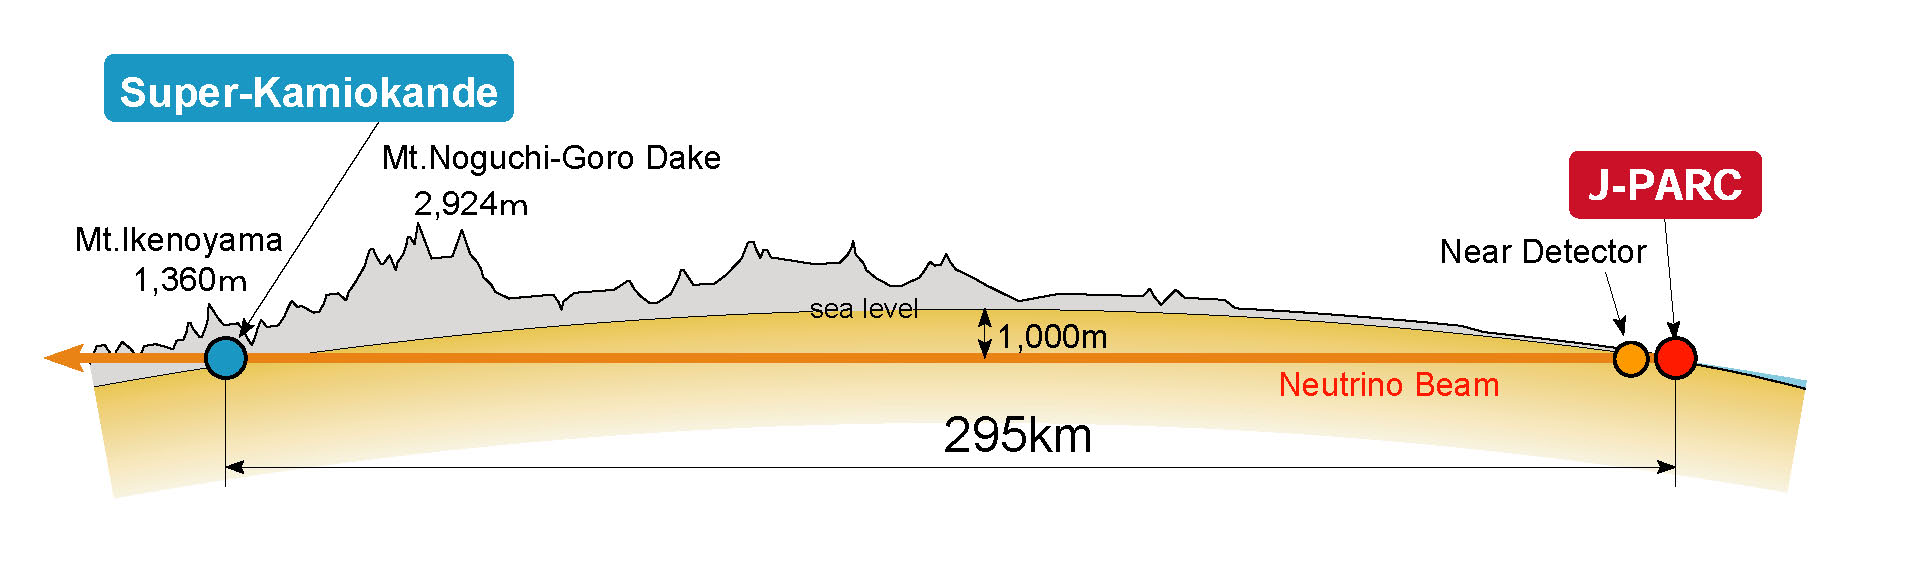
\includegraphics[width=1.0\textwidth, trim={0mm 0mm 0mm 0mm}, clip,page=1]{figures/det_chap/view/t2k_overview}
	\caption{The T2K experiment where neutrinos are created at the J-PARC complex in Tokai and the neutrino beam is characterised at the near-detectors 280 m downstream. 295 km west is the Super-Kamiokande far-detector, measuring the oscillated neutrino spectrum}
	\label{fig:t2k_overview}
\end{figure}
The neutrinos at T2K come from particle decays---primarily $K^\pm$, $\pi^\pm$ and $\mu^\pm$---after a proton beam impinges on a target at the J-PARC complex. The neutrino direction is measured by a suite of near-detectors $\sim280$ m downstream of the target and a muon monitor, providing information on the neutrino flux, directionality and interaction cross-section. One near-detector, INGRID, is a plastic scintillator and iron sandwiched detector placed on-axis, extends $\pm1\deg$ in a cross as to measure the neutrino flux and directionality, and is detailed in \autoref{sec:ingrid}. A second near-detector, ND280, sits $2.5\deg$ off-axis and is surrounded by a 0.1T magnetic field and consists of sub-detectors with multiple interaction targets and a tracker region, designed to accurately measure neutrino interactions under a similar neutrino flux to Super-Kamiokande, and is detailed in \autoref{sec:nd280}. The far detector, Super-Kamiokande, sits 295 km downstream of the target station and measures the rate of neutrino interactions on its 50,000 tonnes of purified water, detailed in \autoref{sec:sk}. A schematic of the travel is shown in \autoref{fig:t2k_overview}.

A host of other neutrino detectors---not used in this analysis---additionally sit in ``pit'' 280m from the target station with ND280 and INGRID. Examples include the liquid emulsion NINJA experiment\cite{ninja}, the water target WAGASCI\cite{wagasci} experiment and its magnetic calorimeter Baby-MIND\cite{baby_mind}. These will in the future make precision measurements of neutrino-nucleus interactions, a dominant systematic for current oscillation analyses.

\begin{figure}[h]
	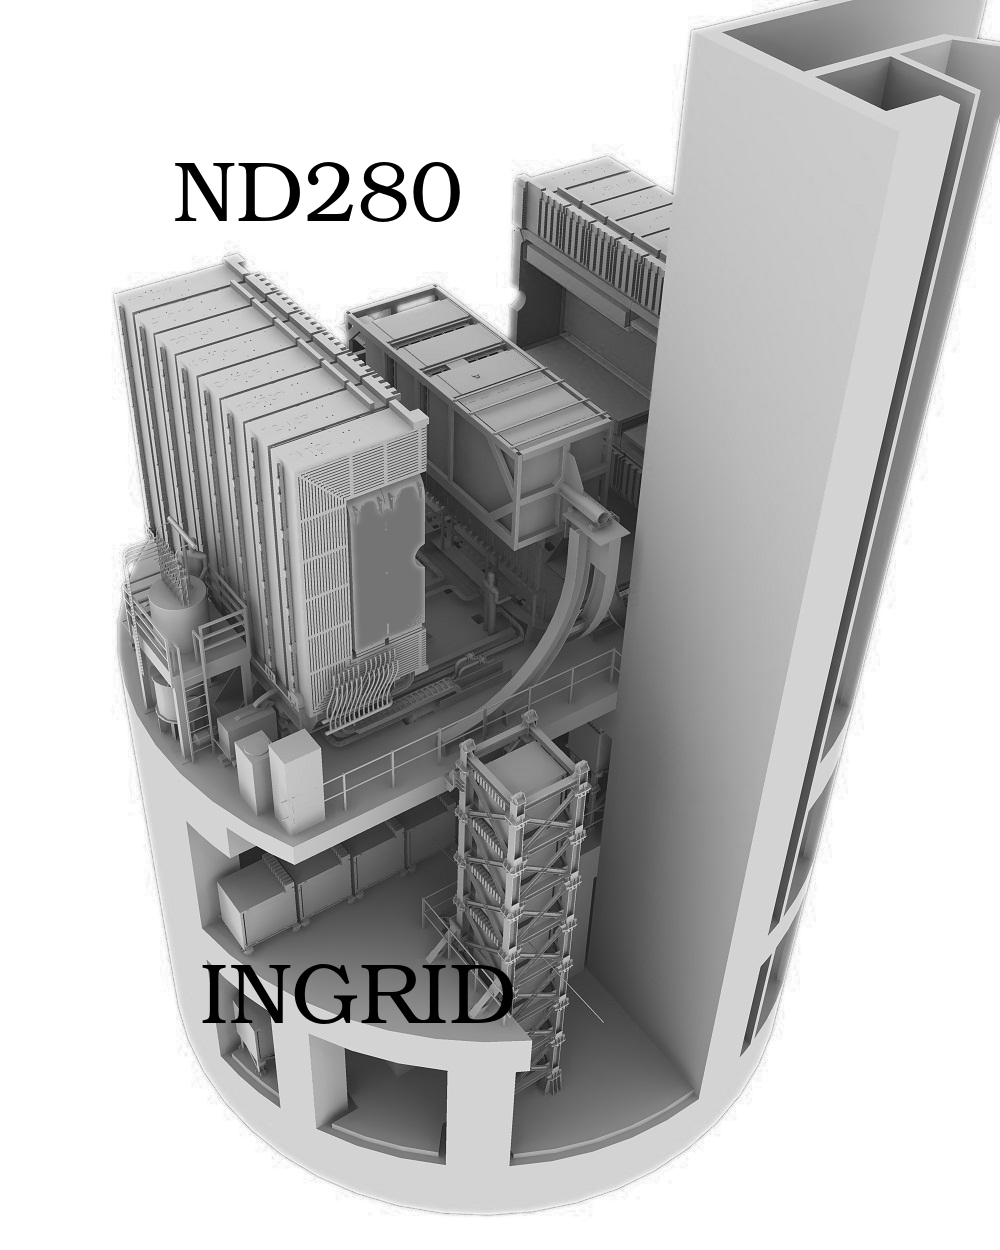
\includegraphics[width=0.4\textwidth, trim={10mm 0mm 0mm 0mm}, clip,page=1]{figures/det_chap/view/image_nd.jpeg}
	\caption{The suite of near-detectors at 280 m from the target, showing ND280 and INGRID}
\end{figure}

\section{Beamline}
The J-PARC complex\cite{jparc_tdr} is used to accelerate protons to 30 GeV/c using a linear accelerator (LINAC), a rapid cycling synchrotron (RCS) and a main ring (MR) synchrotron. The MR has the ability to fast-extract into the neutrino beamline with a design power of 750kW at 30 GeV/c, using $\sim3\times10^{14}$ protons per spill with 8 proton bunches per spill, with a spill cycle of $\sim0.5$Hz. The spill width, which opens the trigger window at the neutrino detectors, is $\sim5\mu$s\cite{t2k_det}.

\begin{figure}[h]
	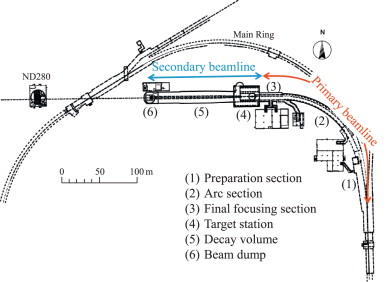
\includegraphics[width=0.4\textwidth, trim={0mm 0mm 0mm 0mm}, clip,page=1]{figures/det_chap/beam/beam.jpg}
	\caption{The neutrino beamline for neutrinos at J-PARC}
	\label{fig:neutrino_beamline}
\end{figure}

The neutrino beamline consists of two parts and is shown in \autoref{fig:neutrino_beamline}: the primary beamline---which takes fast-extracted protons from the MR, bends them to point towards SK, and impinges them on a graphite target---and the secondary beamline---which transports the mesons from the proton-target interactions through a decay volume, finishing with a beam dump. Shortly after the target in the secondary beamline are three magnetic horns\cite{t2k_horns} which are used to deflect (focus) wrong-sign (right-sign) mesons to reduce (enhance) wrong-sign (right-sign) neutrinos. Running the magnets at 250 kA (1.7 T) increases the neutrino flux at SK by factor $\sim17$\cite{t2k_beam}. After running through the magnets, the focused mesons pass through a $\sim96$m decay volume in which the majority of them decay. Particles then strike the beam dump, which stops all mesons. Surviving high momentum muons $p_\mu > 5.0 \text{ GeV/c}$ generally pass through the beam dump, after which they are measured by muon monitors. The muon monitors measure the neutrino beam direction to better than 0.25 mrad and the beam intensity better than 3\%\cite{t2k_mumon,t2k_mumon2}, and is used to inform the beam simulation group.

The neutrinos come primarily from three meson decays
\begin{align*}
	\pi^+ & \rightarrow \mu^+ + \nu_\mu 		&  99.99\% 			& & K^+ & \rightarrow \mu^+ + \nu_\mu 			& 63.6\% & & K^0_L & \rightarrow \pi^- + e^+ + \nu_e 	  & 40.6\% \\
	      & \rightarrow e^+ + \nu_e 			&  10^{-4}\%		& &		& \rightarrow \pi^0 + e^+ + \nu_e 		& 5.1\%  & &	   & \rightarrow \pi^- + \mu^+ + \nu_\mu &  27.0\% \\
	      & \rightarrow \mu^+ + \nu_\mu + \gamma & 2\times 10^{-4}\%  & &		& \rightarrow \pi^0 + \mu^+ + \nu_\mu  	& 3.5\%  & &	   & & 		 &
\end{align*}

\iffalse
\begin{align*}
	\pi^+ 	& \rightarrow \mu^+ + \nu_\mu & 0.9999\\
			& \rightarrow e^+ + \nu_e 	  & 0.0001\\
	K^+   	& \rightarrow \mu^+ + \nu_\mu & 0.6355\\
			& \rightarrow \pi^0 + \mu^+ + \nu_\mu & 0.0353\\
			& \rightarrow \pi^0 + e^+ + \nu_e & 0.0507\\
	K^0_L 	& \rightarrow \pi^- + \mu^+ + \nu_\mu & 0.2704\\
			& \rightarrow \pi^- + e^+ + \nu_e & 0.4055
\end{align*}
\fi
and one leptonic decay\cite{pdg_2017}
\begin{align*}
\mu^+ \rightarrow e^+ + \bar{\nu}_\mu + \nu_e & & 100\%
\end{align*}

From the beam simulation we can also trace back each neutrino's parent meson, shown in \autoref{fig:flux_parents}. The two-body $\pi$ parent is clearly dominant for both the \numu and \numubar fluxes, although the higher energy portion ($E_\nu > 3\text{ GeV}$) consists of neutrinos whose parents are $K$. The \nue and \nuebar components of the neutrino beam come primarily from the leptonic $\mu$ decay below $E_\nu = 1 \text{ GeV}$ and then from $K^+$ and $K^0_L$ at $E_\nu = 2 \text{ GeV}$, which are all three-body decays. Tertiary decay products, e.g. a $\pi^-$ from a $K^0_L$ decay, form large portions of the wrong-sign background.
\begin{figure}[h]
	\begin{subfigure}[t]{0.32\textwidth}
		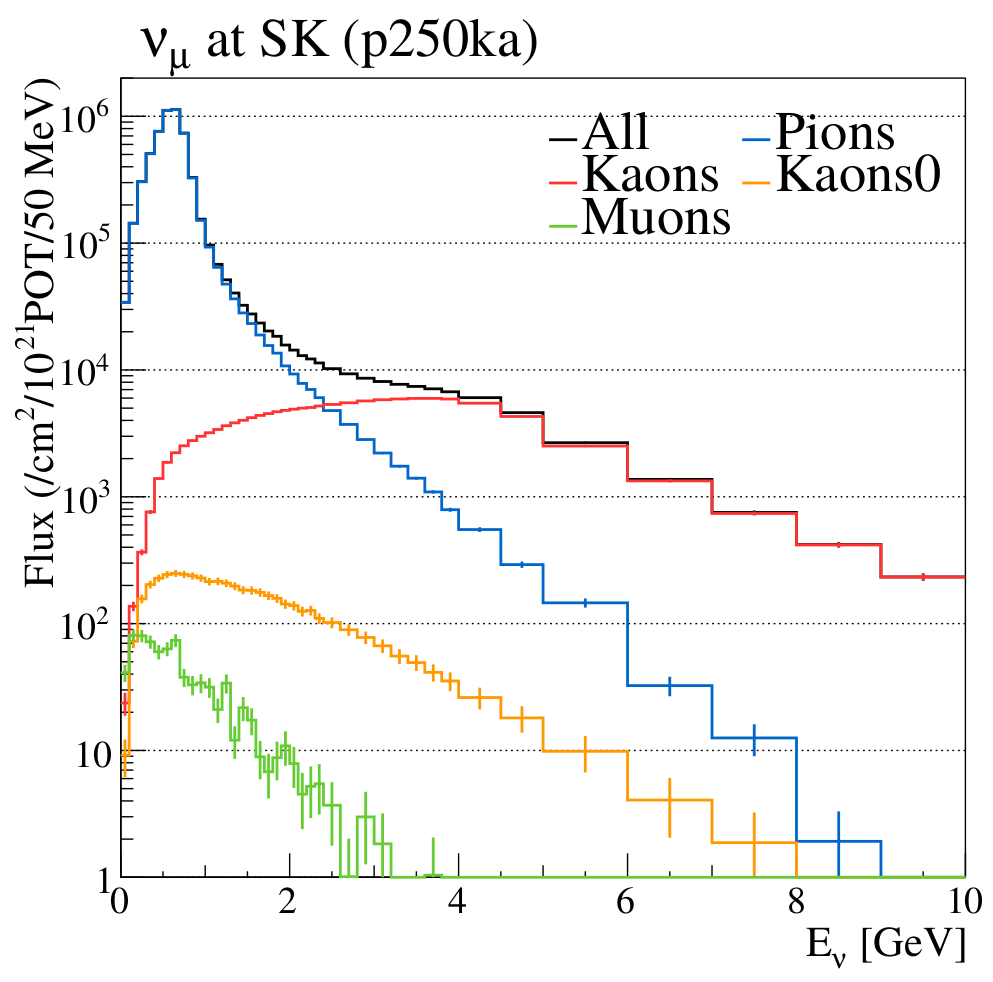
\includegraphics[width=\textwidth, trim={0mm 0mm 0mm 0mm}, clip,page=1]{figures/det_chap/beam/numu_sk_parents}
	\end{subfigure}
	\begin{subfigure}[t]{0.32\textwidth}
		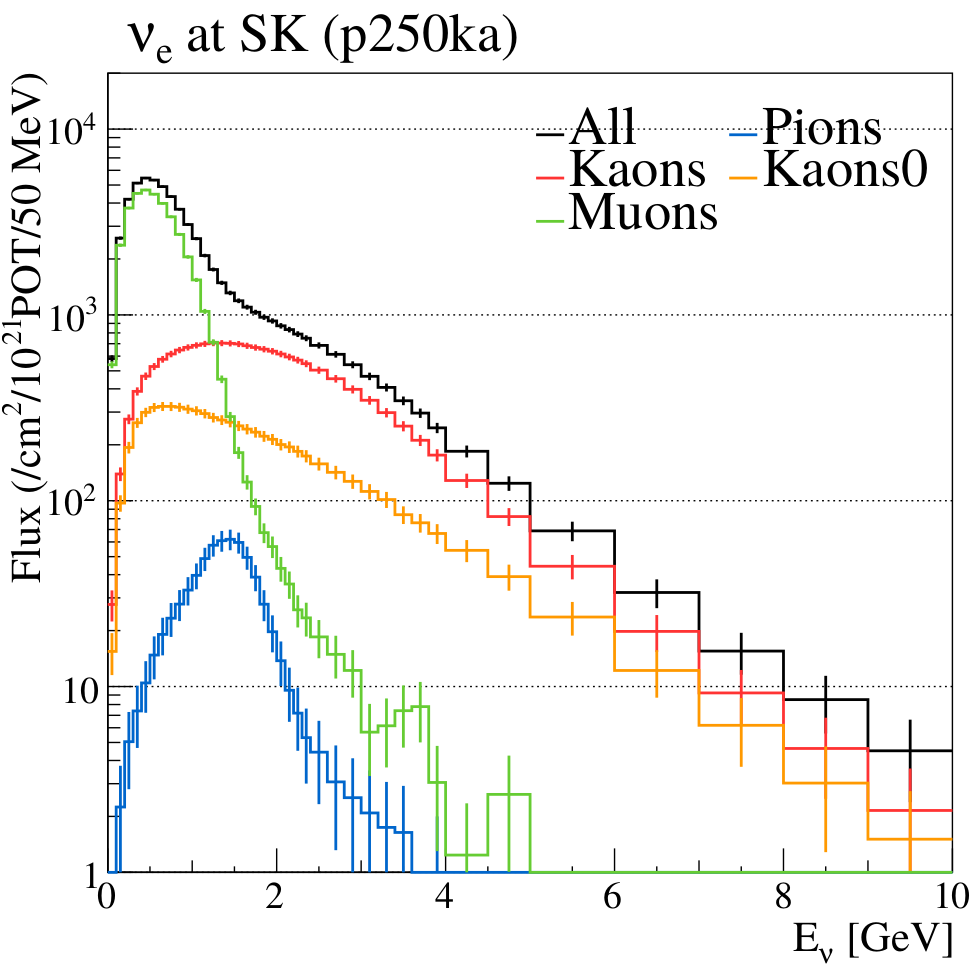
\includegraphics[width=\textwidth, trim={0mm 0mm 0mm 0mm}, clip,page=1]{figures/det_chap/beam/nue_sk_parents}
	\end{subfigure}

	\begin{subfigure}[t]{0.32\textwidth}
		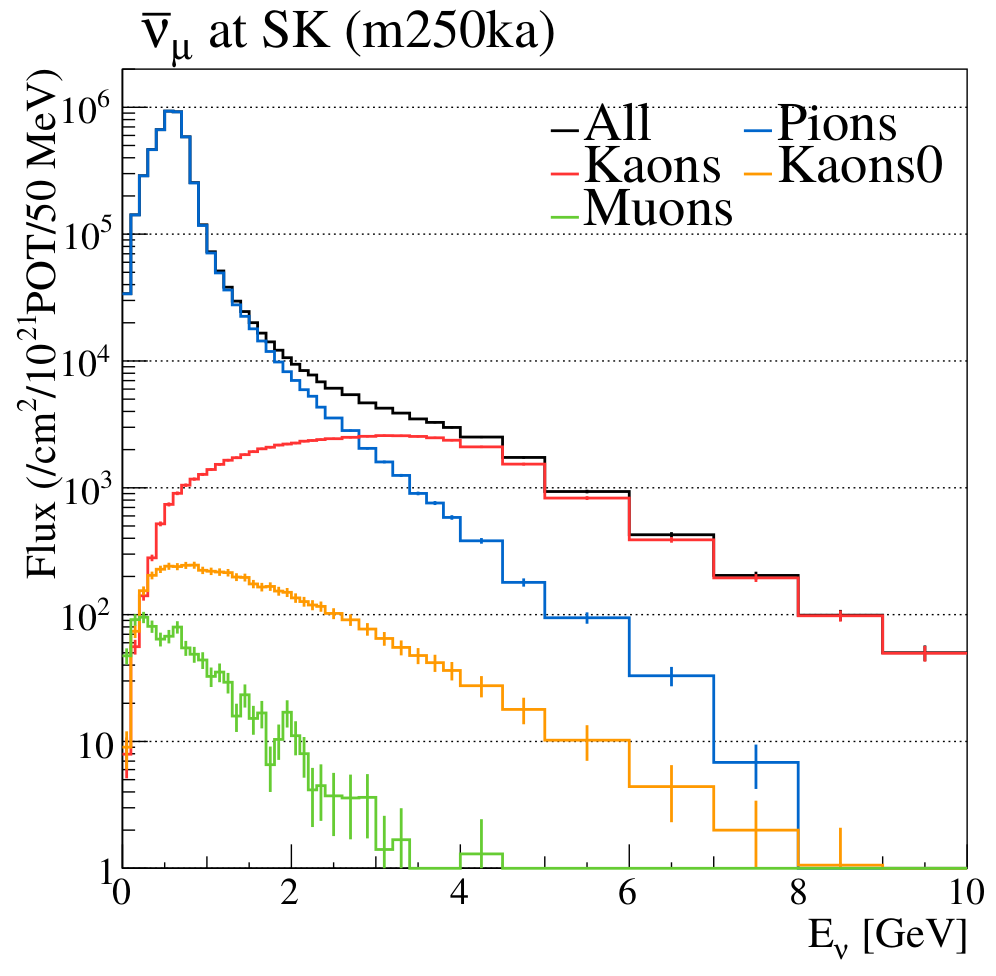
\includegraphics[width=\textwidth, trim={0mm 0mm 0mm 0mm}, clip,page=1]{figures/det_chap/beam/numubar_sk_parents}
	\end{subfigure}
	\begin{subfigure}[t]{0.32\textwidth}
		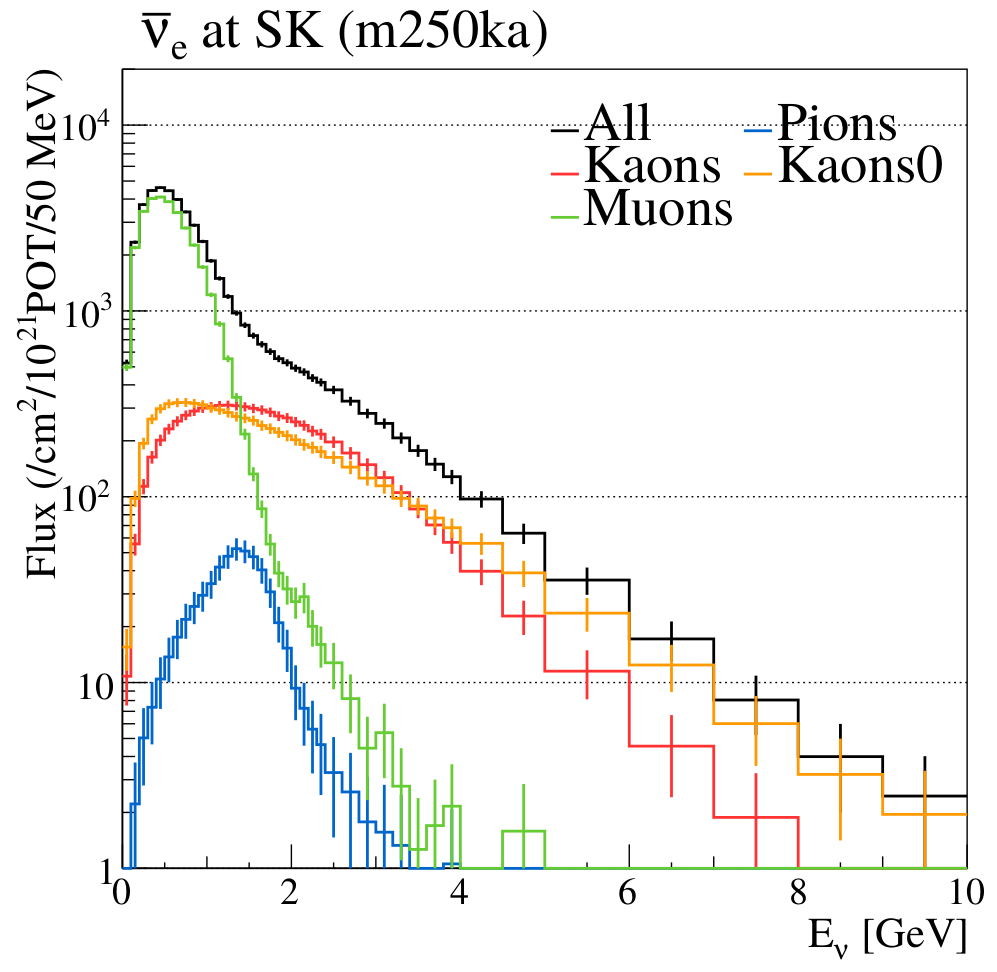
\includegraphics[width=\textwidth, trim={0mm 0mm 0mm 0mm}, clip,page=1]{figures/det_chap/beam/nuebar_sk_parents}
	\end{subfigure}
	\caption{Simulated right-sign neutrino fluxes at SK, showing parents}
	\label{fig:flux_parents}
\end{figure}

The software suite for the beam simulation consists of FLUKA2011 \cite{fluka2008_1, fluka2008_2, fluka2011} which simulates hadronic interactions in target and baffle, JNUBEAM (GEANT3-based \cite{geant3}) which simulates the geometry and tracking, and GCALOR \cite{gcalor} which simulates hadronic re-interactions and is used as a cross-check for FLUKA\cite{t2k_beam, t2k_tn_flux}.

T2K was the first long baseline experiment to use the ``off-axis'' technique\cite{off_axis} in which the far-detector is offset from the neutrino beam center. This has two main effects: 1) it focuses the neutrino energy spectra into a narrower ``peak'' (albeit with lower overall rate than on-axis) and 2) it reduces the wrong-sign background for $\nu_e$ appearance searches. The effect, overlaid with the expected $\nu_\mu$ and $\nu_e$ neutrino flux at Super-Kamiokande is shown in \autoref{fig:off-axis}. Since the neutrino parents are mostly from $\pi$ decay, we can approximately express the neutrino energy $E_\nu$ as a function of pion-neutrino angle $\theta_{\pi,\nu}$, pion energy $E_\pi$ and mass $m_\pi$ and the muon mass $m_\mu$,
\begin{equation}
	E_\nu = \frac{m^2_\pi-m^2_\mu}{2\left( E_\pi - p_\pi \cos \theta_{\pi,\nu} \right)} 
\end{equation}

For a chosen $\cos \theta_{\pi,\nu}$, there is a maximum pion energy of $E_\pi^\text{max} = p_\pi/cos\theta_{\pi,\nu}$, giving rise to a maximum neutrino energy of
\begin{equation}
	E_\nu^\text{max} = \frac{m^2_\pi-m^2_\mu}{2E_\pi \sin^2 \theta_{\pi,\nu}} 
\end{equation}

which maximises when $\pi$ and $\nu$ are near collinear, and as $\theta$ increases the allowed neutrino energy spectrum becomes smaller. The calculated flux at SK with the neutrino oscillation probability is shown in \autoref{fig:off-axis}. The off-axis angle is chosen to maximise the flux in the primary oscillation dip at $E_\nu \sim 0.6\text{ GeV}$.
\begin{figure}[h]
	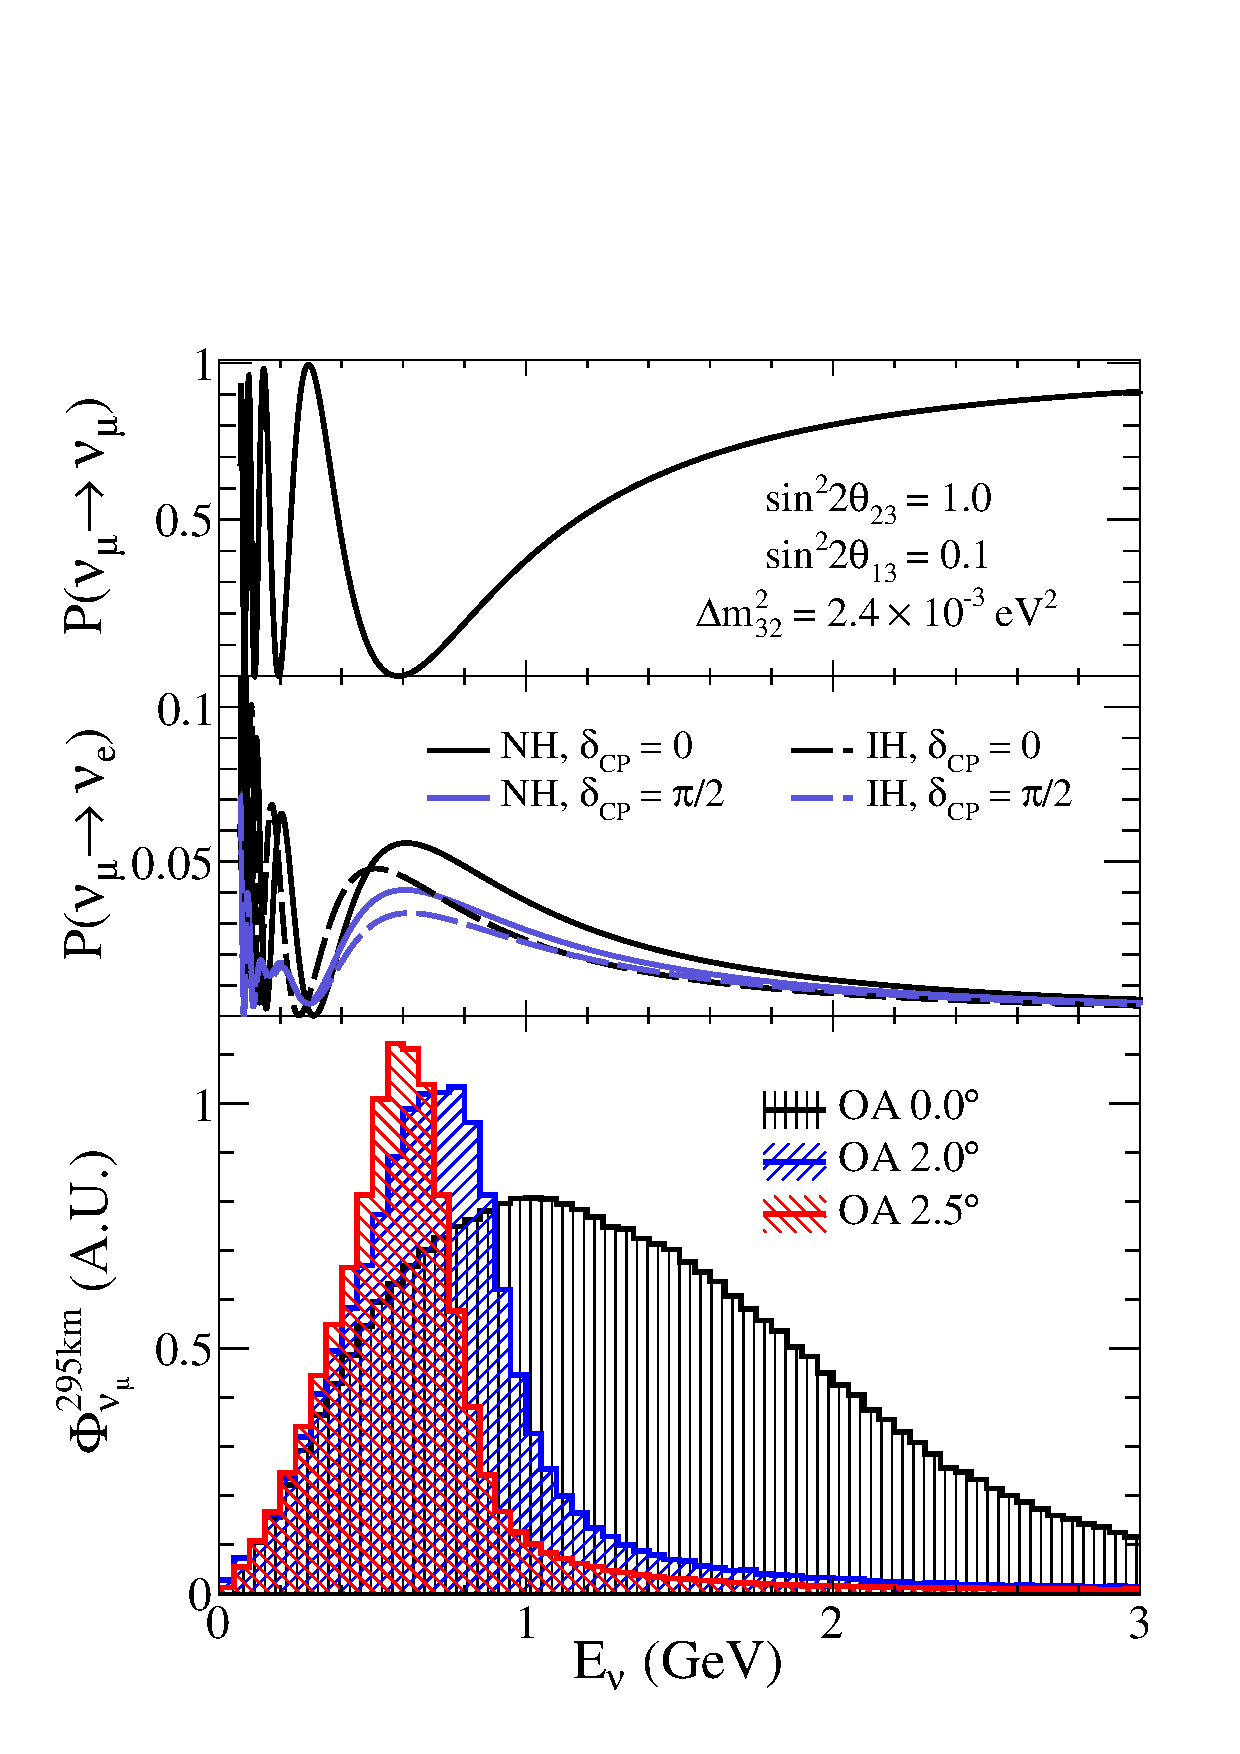
\includegraphics[width=0.4\textwidth, trim={0mm 0mm 0mm 0mm}, clip,page=1]{figures/det_chap/oaeffect_pnue_pnumu_flux}
	\caption{Effect of off-axis (OA) angle on the SK neutrino flux}
	\label{fig:off-axis}
\end{figure}

The beam power and accumulated POT has been steadily increasing from run 1 in 2010 and run 9 in 2019 finished with $\sim500\text{ kW}$ beam power, accumulating a total of $\sim3.16\times 10^{21}$ POT: $1.51\times 10^{21}$ in FHC and $1.65\times 10^{21}$ in RHC modes.
\begin{figure}[h]
	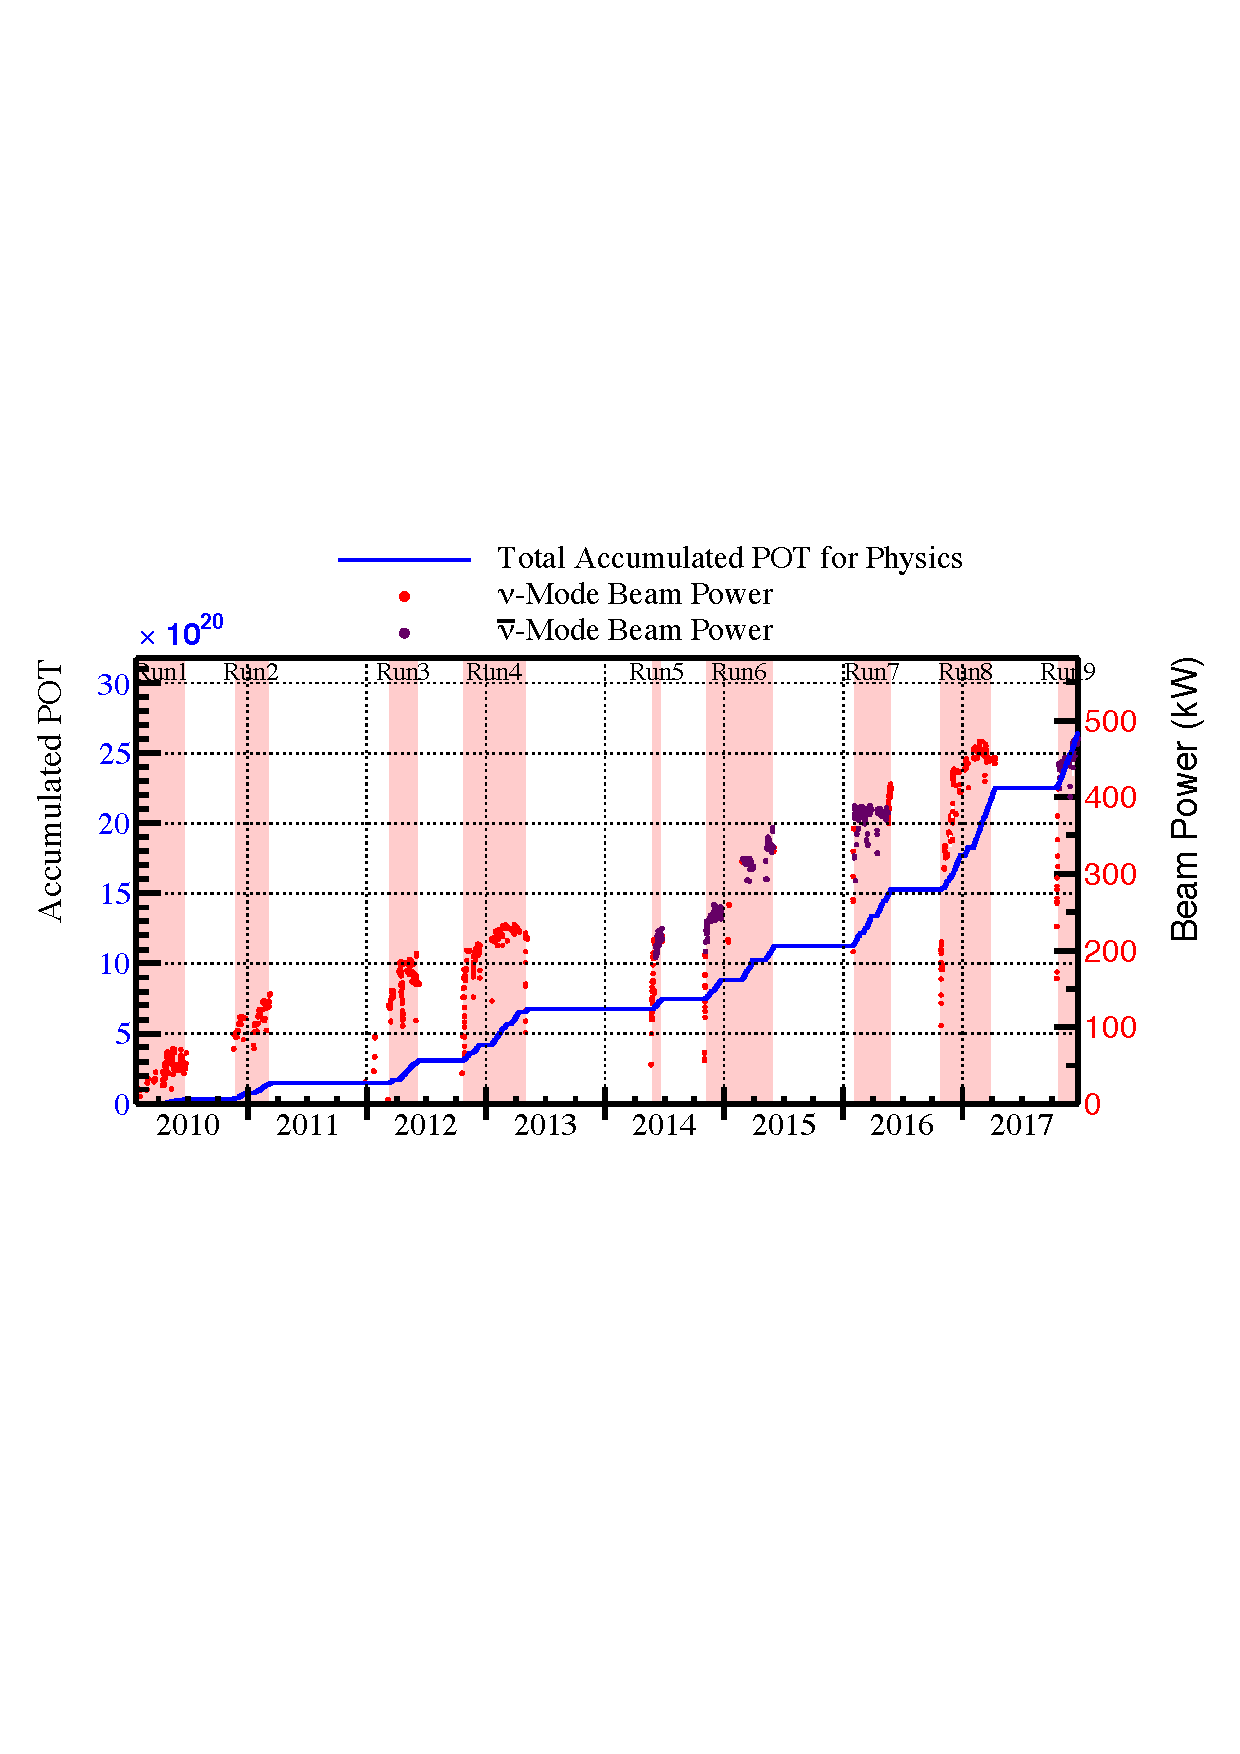
\includegraphics[width=0.5\textwidth, trim= {7mm 40mm 7mm 12mm}, clip]{{figures/pow_t2k_all_toRun77full}}
	\caption{T2K protons on target and beam power for run 1-9}
	\label{fig:t2k_pot}
\end{figure}

The final simulated neutrino fluxes for run 2 to 8 at ND280 are shown in \autoref{fig:flux_1to8}. The wrong-sign background in FHC is $\sim18\%$ which in reality reduces further due to the lower anti-neutrino interaction cross-section, and the \nue component is less than 1\% in the flux peak. The right-sign flux in RHC is very similar to the \numu in FHC, and the majority of the contamination in event rates comes from the cross-section rather than the flux.
\begin{figure}[h]
	\begin{subfigure}[t]{0.45\textwidth}
		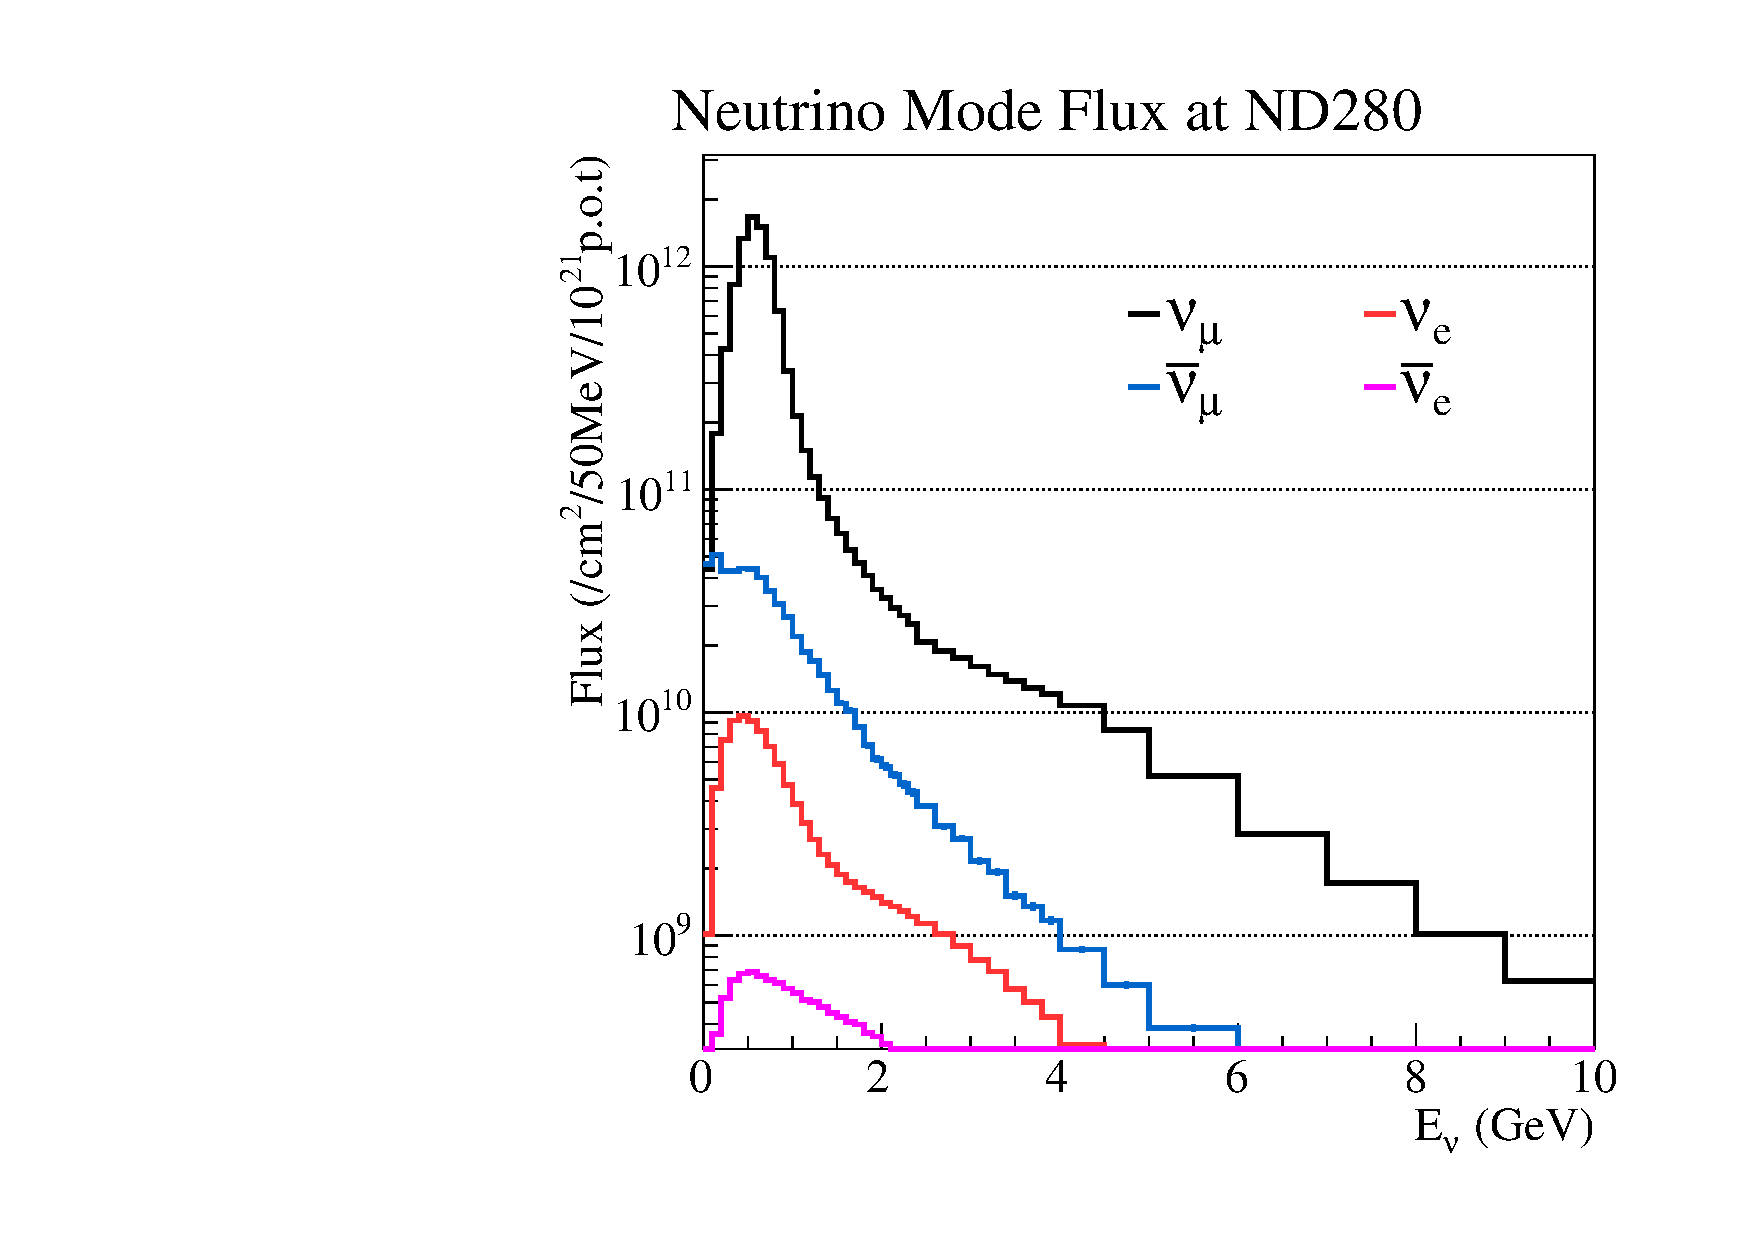
\includegraphics[width=\textwidth, trim={0mm 0mm 0mm 0mm}, clip,page=1]{figures/det_chap/beam/nd5_alltunedflux_run1-8_zoomed_13a}
		\caption{FHC}
	\end{subfigure}
	\begin{subfigure}[t]{0.45\textwidth}
		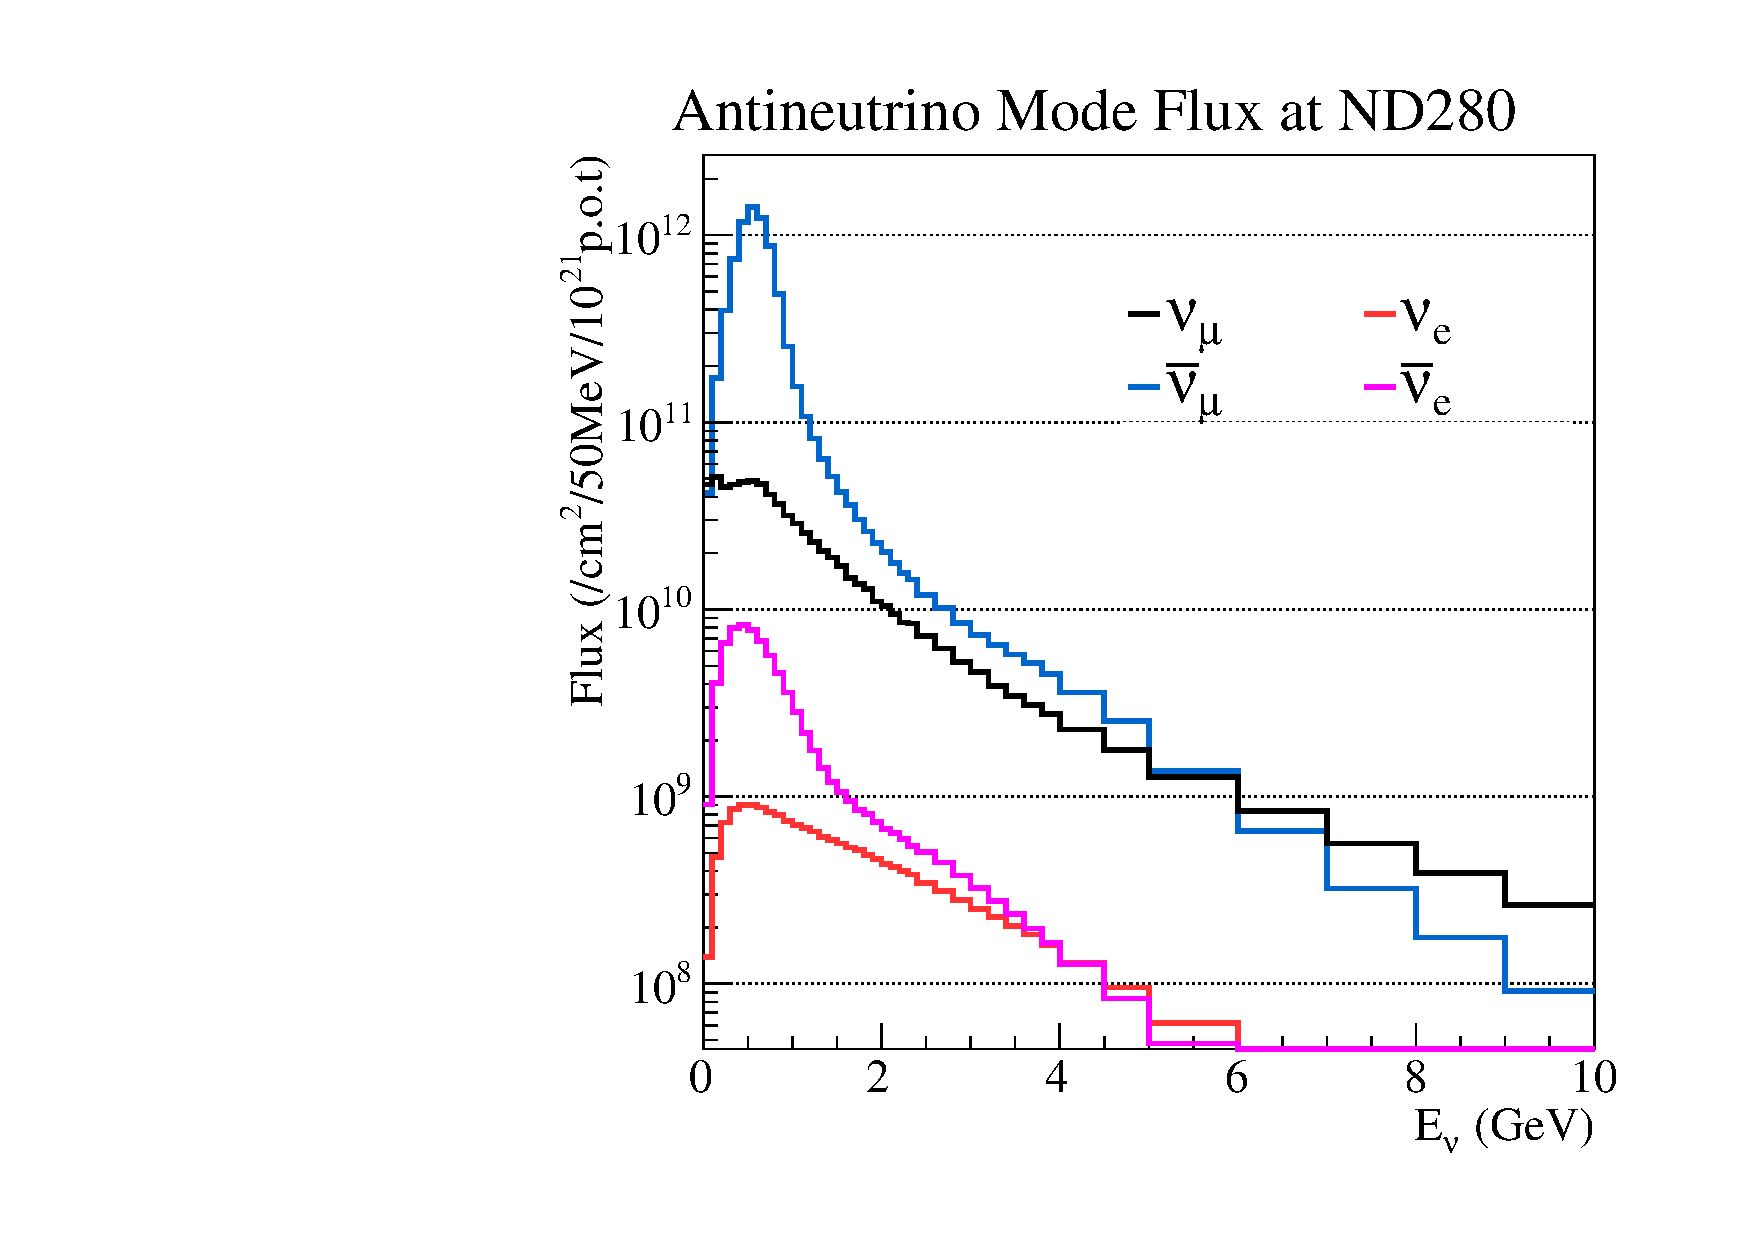
\includegraphics[width=\textwidth, trim={0mm 0mm 0mm 0mm}, clip,page=1]{figures/det_chap/beam/nd5_alltunedflux_run5c-7b_zoomed_antinu_13a}
		\caption{RHC}
	\end{subfigure}
	\caption{Simulated neutrino fluxes at ND280 in forward (FHC) and reverse (RHC) horn current modes}
	\label{fig:flux_1to8}
\end{figure}

\section{INGRID}
\label{sec:ingrid}

\begin{figure}[h]
	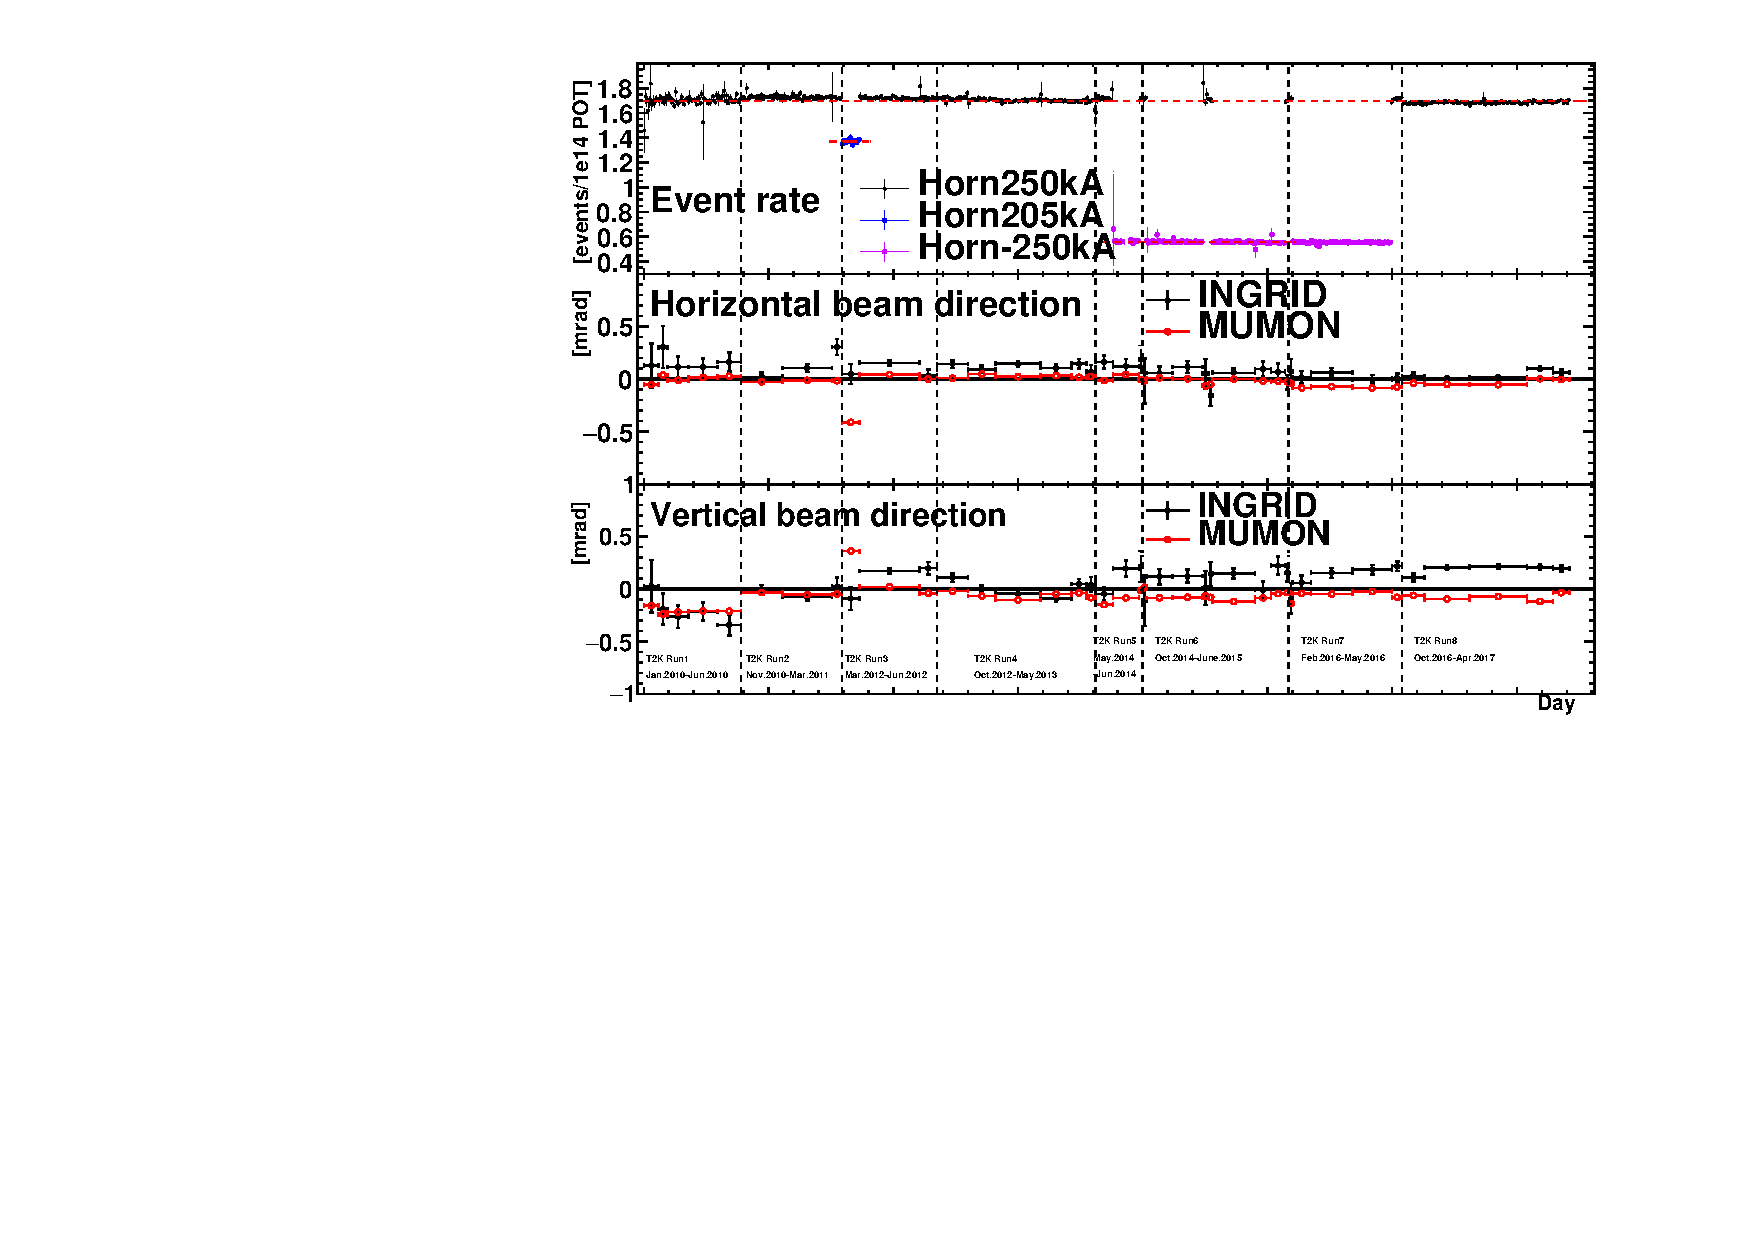
\includegraphics[width=0.4\textwidth, trim={0mm 0mm 0mm 0mm}, clip,page=1]{figures/det_chap/INGRID_official_plot_until74}
	\caption{Beam characteristics measured by the INGRID and MUMON detectors over the full T2K run 1 to 8}
	\label{fig:ingrid_monitoring}
\end{figure}


\cite{t2k_ingrid}
0.4mrad, event rate 4\% precision.

\section{ND280}

\cite{t2k_det}

\label{sec:nd280}
\cite{t2k_det}

\subsection{FGD}
\cite{t2k_fgd}
\subsection{TPC}
\cite{t2k_tpc}
\subsection{ECal}
\cite{t2k_ecal}
\subsection{P0D}
\cite{t2k_p0d}
\subsection{Magnet}

\subsection{SMRD}
\cite{t2k_smrd}

\section{Super Kamiokande}
\label{sec:sk}
\cite{t2k_sk, t2k_sk2, t2k_sk3}

